\section{Edge Detection}\label{edge-detection}

\subsection{Filters and Convolution}\label{filters-and-convolution}

以下只考虑线性、时不变的系统/滤波器，也即\textbf{线性性}（齐次性 $a x(t)\to a y(t)$；
可加性 $x_1(t)+x_2(t)\to y_1(t)+y_2(t)$）与\textbf{时不变性}（$x(t-\tau)\to y(t-\tau)$）。

\subsubsection{1D Filter: Moving Average}\label{d-filter-moving-average}

移动平均就是选取一定的窗口大小，每个输出点是窗口中像素值的加权和。
用卷积表示即： \[
  h[n] = (f * g)[n] = \sum_{k=-K}^{K} f[n-k] \cdot g[k]
\] 其中 \(g[k]\) 是滤波器权重。

\subsubsection{Convolution and Flourier
  Transformer}\label{convolution-and-flourier-transformer}

\textbf{Discrete Signal}：

离散卷积： \[
  (f * g)[n] = \sum_{m=-\infty}^{\infty} f[m]\, g[n-m]
\]

离散傅里叶变换： \[
  \mathcal{F}\{f\}(\omega) = \sum_{n=-\infty}^{\infty} f[n]\, e^{-i2\pi\omega n}
\]

\textbf{Continuous Signal}：

连续卷积： \[
  (f * g)(x) = \int_{-\infty}^{\infty} f(t)\, g(x   - t)\, dt
\]

连续傅里叶变换： \[
  \mathcal{F}\{f\}(\omega) = \int_{-\infty}^\infty f(t)\, e^{-i2\pi \omega t}\, dt
\]

\textbf{Convolution Theory}：

\[
  \mathcal{F}\{f * g\} = \mathcal{F}\{f\} \cdot \mathcal{F}\{g\}
\]
也即\textbf{时域卷积等于频域相乘}。

\subsubsection{2D Filter: Moving
  Average}\label{d-filter-moving-average-1}

选取一定的窗口大小，每个输出点是窗口中像素的加权和。 卷积表示： \[
  (f * g)[m,n] = \sum_{k}\sum_{\ell} f[k,\ell]\, g[m-k,\, n-\ell]
\]

\subsubsection{Gaussian Filter}\label{gaussian-filter}

高斯滤波是一种常用的低通滤波器。

\paragraph{1D}\label{d}

时域： \[
  g(x) = \frac{1}{\sqrt{2\pi}\,\sigma} \exp\left(-\frac{x^2}{2\sigma^2}\right)
\]

频域： \[
  \mathcal{F}\{g\}(\omega) = \exp\left(-\frac{\sigma^2 \omega^2}{2}\right)
\]

\paragraph{2D}\label{d-1}

空域： \[
  g(x,y) = \frac{1}{2\pi\sigma^2} \exp\left(-\frac{x^2 + y^2}{2\sigma^2}\right)
\]

频域： \[
  \mathcal{F}\{g\}(\omega_x, \omega_y) = \exp\left(-\frac{\sigma^2 (\omega_x^2 + \omega_y^2)}{2}\right)
\]

显然在频域仍为 Gaussian 分布。故 \(\sigma\)
越大，频域越锋利，选择的低频成分越多。

\subsection{Edge Detection}\label{edge-detection-1}

\subsubsection{The Definition of Edges}\label{the-definition-of-edges}

边缘的数学定义由\textbf{梯度}给出：边缘上，梯度的幅值应当在梯度方向上取得局部极大值，且在梯度的正交方向上基本不变。

梯度向量： \[
  \nabla f(x,y) = \left(\frac{\partial f}{\partial x}, \frac{\partial f}{\partial y}\right)
\] 梯度幅值（magnitude）： \[
  |\nabla f| = \sqrt{\left(\frac{\partial f}{\partial x}\right)^2 + \left(\frac{\partial f}{\partial y}\right)^2}
\] 梯度方向（orientation）： \[
  \theta = \operatorname{atan2} \left(\frac{\partial f}{\partial y}, \frac{\partial f}{\partial x}\right)
\]

\subsubsection{Criteria for Edge
  Detection}\label{criteria-for-edge-detection}

边缘检测本质上是一个\textbf{二分类问题}，因此可以用以下指标评价：

\textbf{精确率}： \[
  \text{Precision} = \frac{TP}{TP + FP}
\] 也即检测出的边缘中，有多少是真正的边缘

\textbf{召回率}： \[
  \text{Recall} = \frac{TP}{TP + FN}
\] 也即真实边缘中，有多少被成功检测出来

三个重要准则：

\begin{enumerate}
  \def\labelenumi{\arabic{enumi}.}
  \tightlist
  \item
        \textbf{Good Detection}：
        尽可能检测出所有真实边缘，尽量避免把噪声检测为边缘。也即\textbf{精确率}和\textbf{召回率}尽量高
  \item
        \textbf{Good Localization}：
        检测到的边缘位置必须尽可能接近真实的边缘位置。也即检测边缘与真实边缘之间的\textbf{距离}尽量小
  \item
        \textbf{Single Response}：
        对于每一条真实的边缘，算法应该只产生\textbf{一个}响应，而不是多个。
\end{enumerate}

\subsubsection{Finite Difference}\label{finite-difference}

连续偏导数在数字图像上用差分近似：

\begin{itemize}
  \tightlist
  \item
        中心差分： \[
          \frac{\partial f}{\partial x}\bigg|_{(m,n)} \approx \frac{f(m+1, n)   - f(m-1,n)}{2}
        \] \[
          \frac{\partial f}{\partial y}\bigg|_{(m,n)} \approx \frac{f(m, n+1)   - f(m,n-1)}{2}
        \]
  \item
        前向/后向差分也可用，但精度稍差： \[
          \frac{\partial f}{\partial x}\bigg|_{(m,n)} \approx f(m+1,n)   - f(m,n)
        \]
\end{itemize}

\subsubsection{Derivative Theorem of
  Convolution}\label{derivative-theorem-of-convolution}

在先平滑后差分时，我们可以利用\textbf{导数定理}进行分步简化计算。

导数定理： \[
  \frac{\partial}{\partial x}(f * g) = f * \frac{\partial g}{\partial x}
\]

这意味着我们可以把先卷积再差分合并成一次卷积（用导数的 Gaussian
kernel），节省计算并更好地控制尺度。

具体地，我们用 x、y 导数 Gaussian 对图像做卷积得到两个分量： \[
  G_x = f * \frac{\partial g}{\partial x}, \qquad G_y = f * \frac{\partial g}{\partial y}
\] 从而计算出梯度幅值与方向： \[
  |\nabla f| = \sqrt{G_x^2 + G_y^2}, \quad \theta = \operatorname{atan2} (G_y, G_x)
\]

\subsubsection{Post Processing}\label{post-processing}

\paragraph{Non-Maximal Suppression}\label{non-maximal-suppression}

非极大值抑制算法，用以形成\textbf{单像素}边缘。

步骤：

\begin{enumerate}
  \def\labelenumi{\arabic{enumi}.}
  \tightlist
  \item
        对每个像素 \(q\) 计算梯度 \(g(q)\) 以及梯度幅值 \(M(q)\)。
  \item
        沿梯度方向向两侧移动到点
        \(q_1 = q + g_{dir}(q)\)，\(q_2 = q   - g_{dir}(q)\)，其中 \(g_{dir}\)
        是归一化梯度向量。
  \item
        使用双线性插值在 \(q_1\)、\(q_2\) 处计算幅值 \(M(q_1)\)、\(M(q_2)\)。
  \item
        若 \(M(q)\) 大于 \(M(q_1)\) 和 \(M(q_2)\)，则保留；否则抑制为 0。
\end{enumerate}

\textbf{双线性插值（bilinear interpolation）}：

给定四个格点
\(Q_{11}=(x1, y1)\)，\(Q_{12}=(x1, y2)\)，\(Q_{21}=(x2, y1)\)，\(Q_{22}=(x2, y2)\)，\(P=(x, y)\)
点的双线性插值为： \[
  f(P) = f(Q_{11}) (1-\alpha)(1-\beta) + f(Q_{21}) \alpha (1-\beta) + f(Q_{12}) (1-\alpha)\beta + f(Q_{22}) \alpha \beta
\] 其中
\(\alpha = \frac{x   - x_1}{x_2   - x_1}\)，\(\beta = \frac{y   - y_1}{y_2   - y_1}\).

本质上就是按照距离整点的距离比例进行加权。

\centering
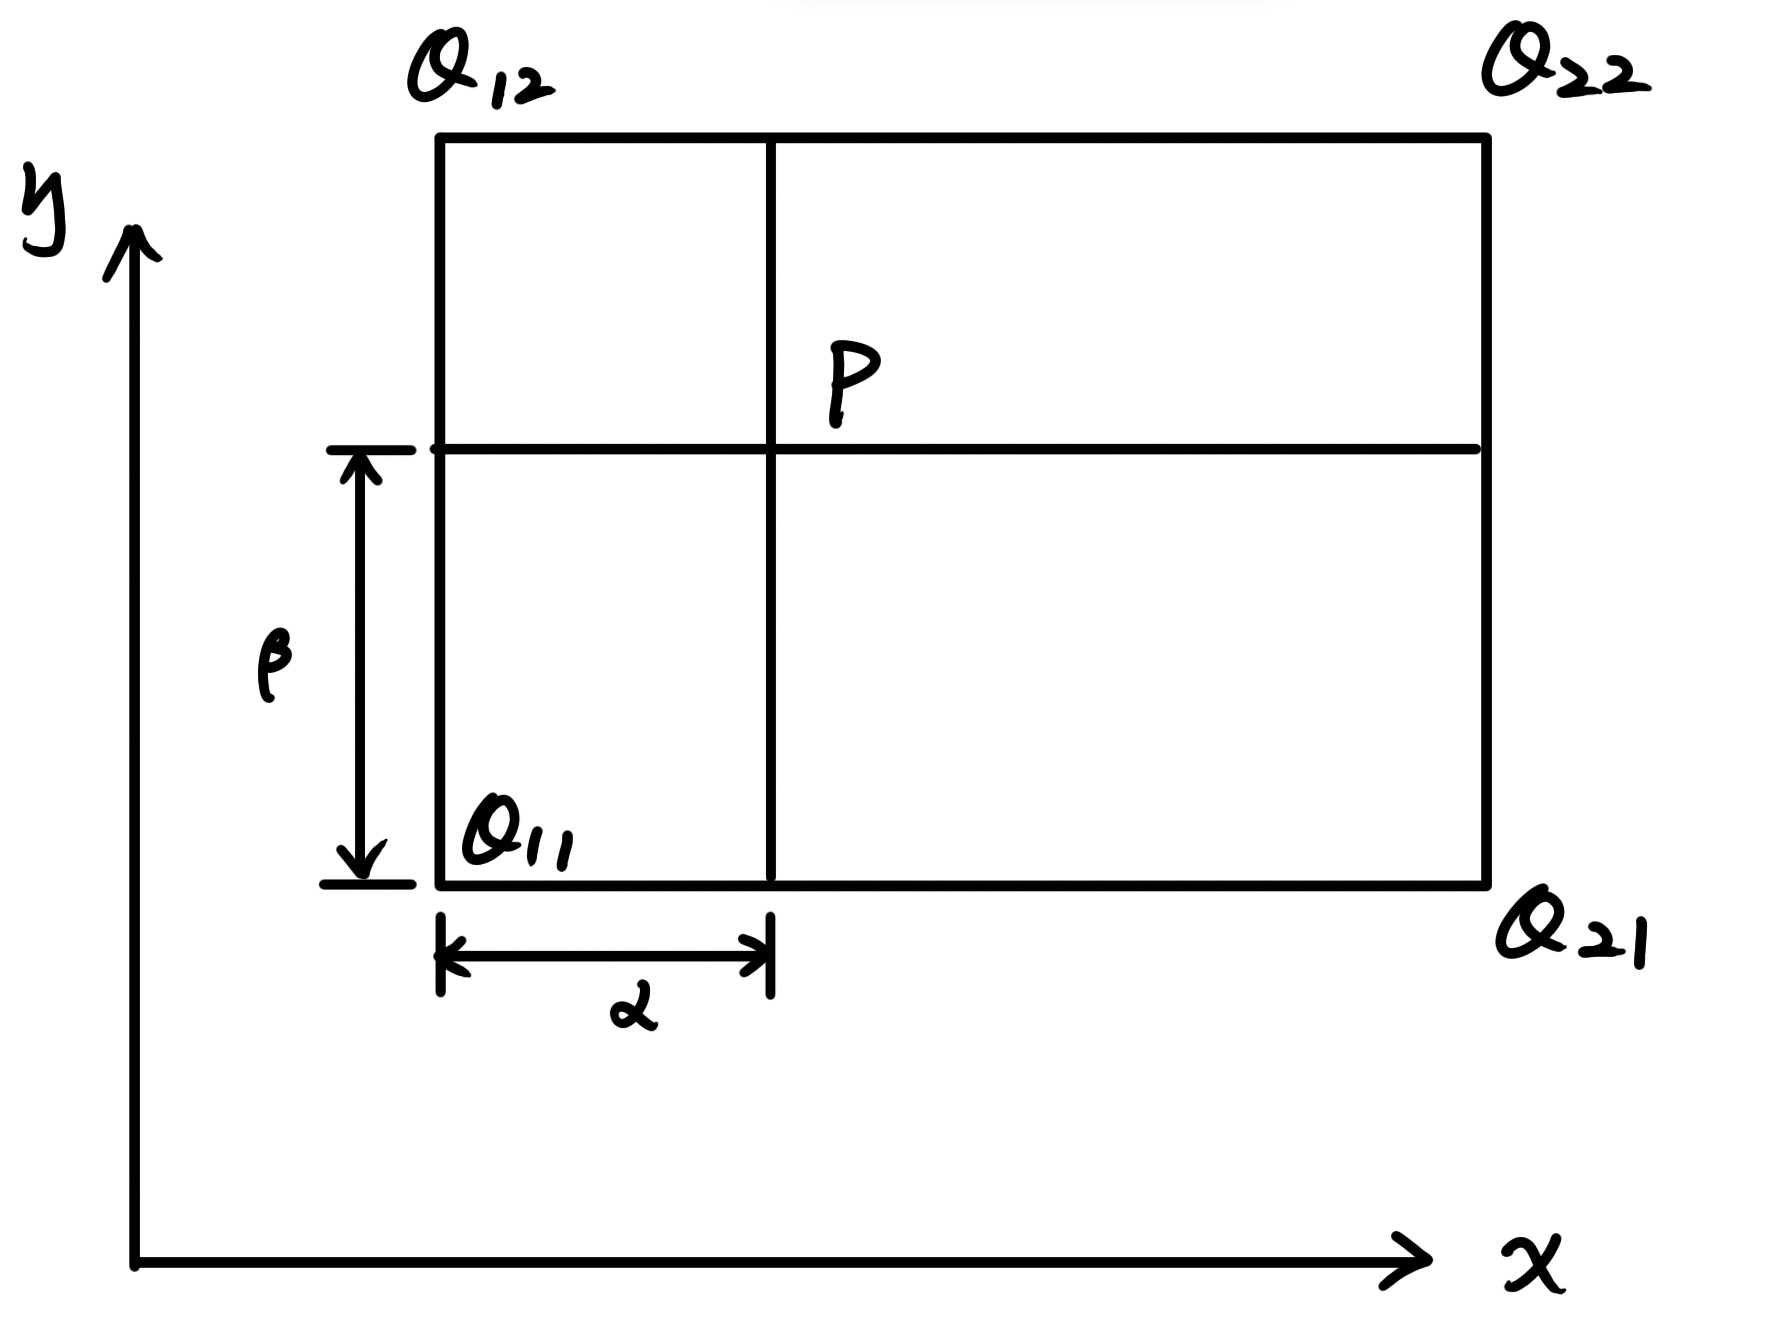
\includegraphics[width=\linewidth]{assets/02-edge-01-bilinear-interpolation.jpg}
\captionof{figure}{图1：双线性插值}

\textbf{简化 NMS}：

离散化为 8 个方向并直接比较相邻像素。

\paragraph{Hysteresis Thresholding}\label{hysteresis-thresholding}

滞后阈值算法，用以形成\textbf{连续}边缘，可以强化边缘并抑制噪声。

首先确定两个阈值：\(maxVal\)，\(minVal\). 可按通过 NMS
的像素平均幅值设定：
\[
  maxVal = 0.3 \times average
  minVal = 0.1 \times average
\]

对于像素点 \(q\)，幅值 \(M(q)\)：

\begin{itemize}
  \tightlist
  \item
        若 \(M(q) \ge maxVal\)：强边缘，保留并允许连接。
  \item
        若 \(M(q) < maxVal\)：非边缘，抛弃。
  \item
        若 \(minVal \le M(q) < maxVal\)：弱边缘，仅在与强边缘连通时保留。
\end{itemize}

边缘增长（Edge Linking）步骤：

\begin{enumerate}
  \def\labelenumi{\arabic{enumi}.}
  \tightlist
  \item
        遍历图像，遇到强边缘开始增长；
  \item
        对当前边缘像素，检查在边缘方向（垂直梯度方向）上的两个相邻像素，若任一像素方向与该像素
        bin 相同、幅值足够、通过 NMS 判定，则将其也标记为边缘，并继续增长；
  \item
        循环直到不能继续增长为止。
\end{enumerate}

\subsubsection{Canny Edge Detector}\label{canny-edge-detector}

上述流程即使标准的 Canny 算法：

\begin{enumerate}
  \def\labelenumi{\arabic{enumi}.}
  \tightlist
  \item
        用导数 Gaussian 计算梯度分量 \(G_x\)、\(G_y\)。
  \item
        计算梯度幅值和方向。
  \item
        非极大值抑制（NMS）将响应细化到单像素宽。
  \item
        使用滞后阈值并做边缘连接（Hysteresis + Edge
        Linking）产生最终的边缘线条。
\end{enumerate}

\textbf{注}：


Canny 算法涉及很多 Hyper Parameter，如
\(\sigma\)、\(maxVal\)、\(minVal\).
其中尺度选择（\(\sigma\)）是关键。\(\sigma\)
大时噪声更少但定位差；\(\sigma\)
小时定位好但对噪声敏感。通常对同一图像做多尺度检测以获得更稳健结果。
